\documentclass[12pt, onecolumn]{IEEEtran}
\usepackage{graphics,  color,  amsmath, amsfonts, amssymb, balance,algorithm,algorithmic,array ,comment}
\usepackage{graphicx}
%\usepackage{bbding}
%\usepackage{multirow}
\usepackage{caption}
\usepackage{algorithm}
\usepackage{algorithmic}
\usepackage{amsmath, amssymb}
\usepackage{mathrsfs}
\usepackage{bm}%Greek letters in boldface
\vfuzz2pt % Don't report over-full v-boxes if over-edge is small draftcls
\hfuzz2pt % Don't report over-full h-boxes if over-edge is small
% THEOREMS -------------------------------------------------------
\newtheorem{thm}{Theorem}%[section] ,draftcls
\newtheorem{cor}{Corollary}
\usepackage{amsthm}
\newtheorem{lem}{Lemma}
\newtheorem{prop}{Proposition}
\newtheorem{defn}{Definition}
\newtheorem{rem}{Remark}
\newtheorem{example}{Example}
\newtheorem{theorem}{Theorem}
\renewcommand{\algorithmicrequire}{ \textbf{Initialization:}}
\renewcommand{\algorithmicensure}{ \textbf{Return:}}

\author{Jianxin Dai\\
}
\title{Users Selection Report }
\begin{document}
\maketitle


\section{Introduction}

In the paper \cite{geraci2017operating}, authors proposed to operate massive Multiple Input Multiple Output (MIMO) cellular Base Stations (BSs) in unlicensed bands (mMIMO-U). they design a procedures required at a cellular BS to guarantee coexistence with nearby WiFi stations in the same piece of unlicensed band via interference alignment technology.  Fig.~\ref{FIG:mMIMO} show the flow of mMIMO-U  proposed.
\begin{figure}[H]
    \centering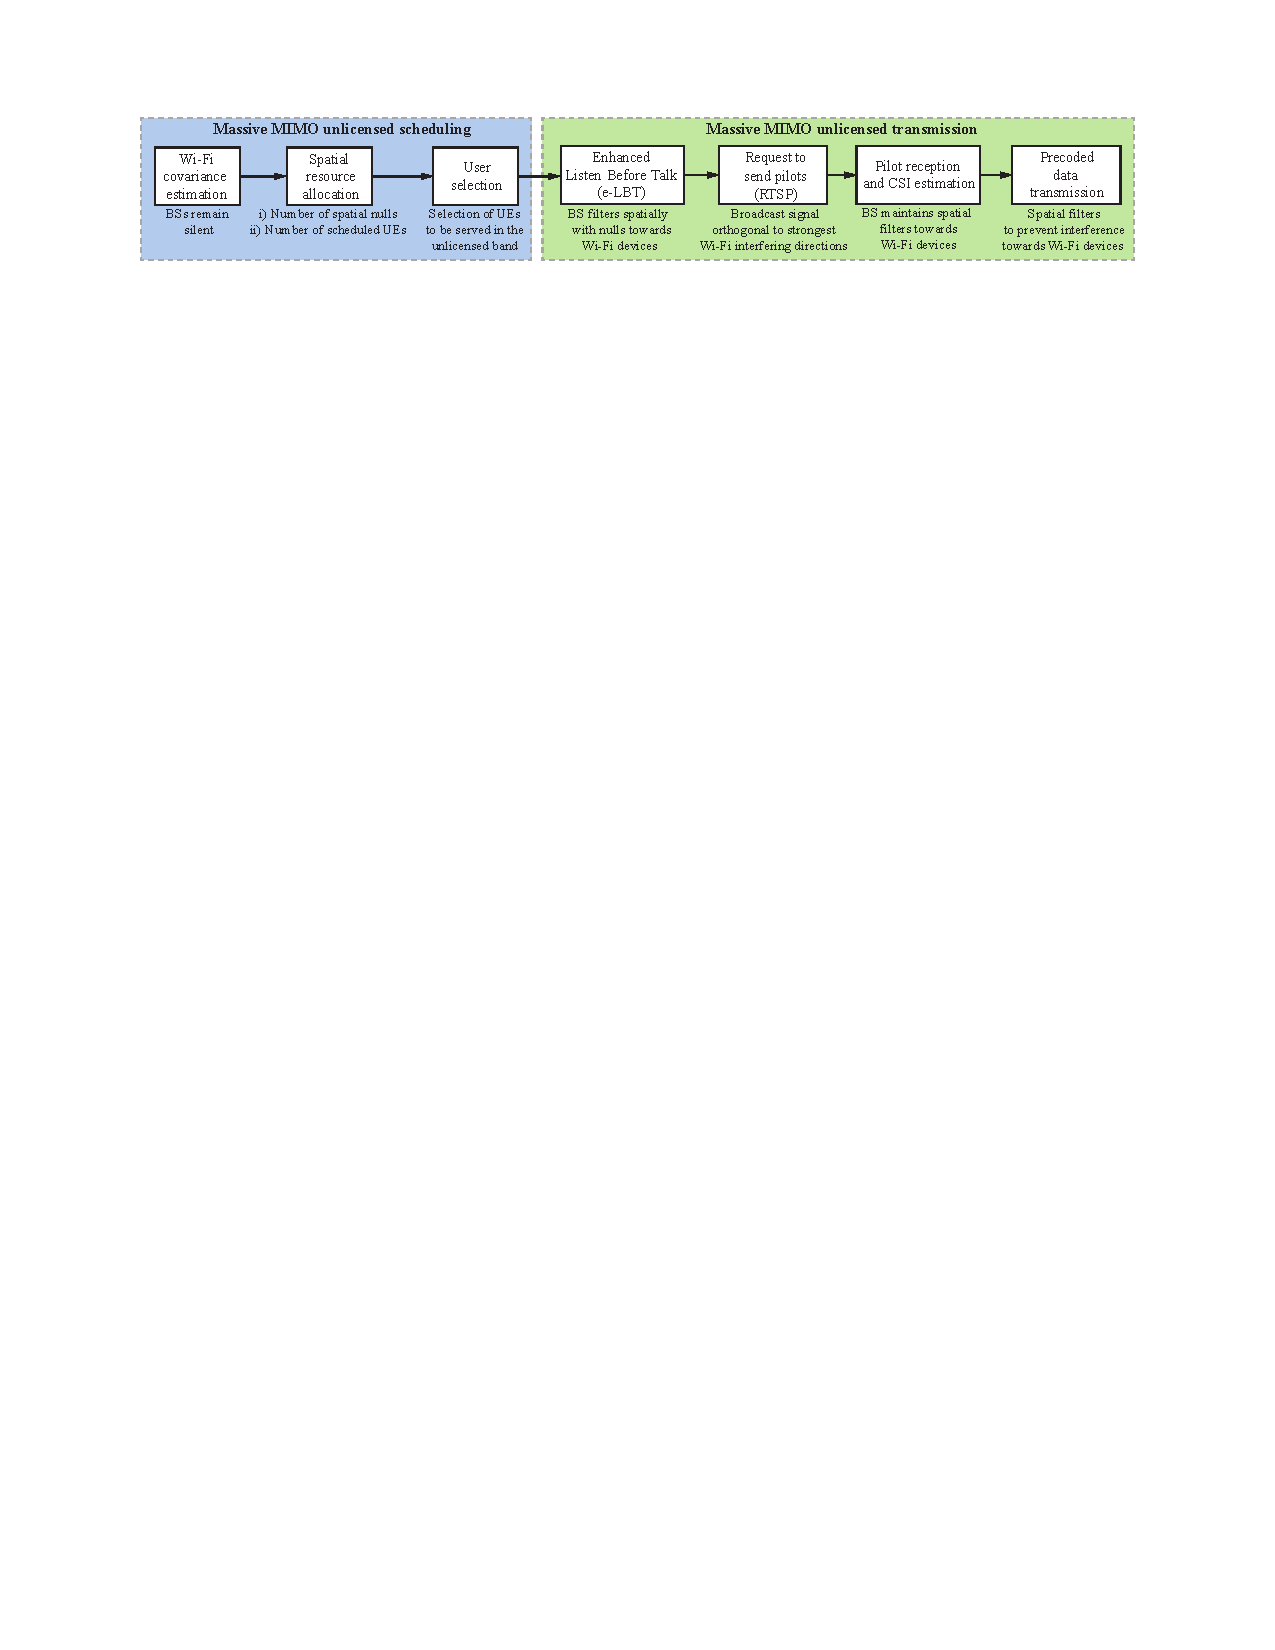
\includegraphics[width=1\columnwidth]{mMIMO.pdf}
    \caption{ Flow chart of the proposed mMIMO-U}\label{FIG:mMIMO}
\end{figure}
\begin{description}
  \item[Step1:] %authors discuss the operations requires for a massive MIMO celluar BS to:
                    \begin{enumerate}
                      \item acquire channel state information from the neighboring WiFi devices.
                      \item allocate spatial resources for WiFi interference suppression and user equipment (UE) multiplexing.
                      \item select a suitable set of UEs to be served in the unlicensed band.
                    \end{enumerate}
  \item[Step2:] %authors devise a transmission operations of a massive MIMO-U system, including:
                    \begin{enumerate}
                        \item an enhanced LBT phase.
                        \item procedures for UE pilot request and channel estimation.
                        \item precoder calculation.
                    \end{enumerate}
\end{description}


\section{System Model}

  WE consider the downlink of a cellular network where  massive MIMO cellular BSs are deployed to operate in the unlicensed band in a synchronous manner, and communicate with their respective sets of connected cellular UEs, while WiFi devices also operate in the same unlicensed band.  Each BSs equipped with  a larger number of antennas $N$, and  simultaneously serves K UEs. Each BS transmit with power $P_{b}$. On the WiFi side, $L$ is denoted by the set of WiFi devices. We assume that all WiFi device transmit with power $P_{w}$.  It worth nothing that both UEs and WiFi devices are equipped with one antenna.
 \begin{equation}\label{EQU:ChannelModel}
    \begin{aligned}
        y_{(i,k)}[m] = & \sqrt{P_{b}}h_{[i,(i,k)]}w_{(i,k)}s_{(i,k)}[m] + \sqrt{P_{b}}\sum_{k'\in{}K_{i}\backslash{}k}h_{[i,(i,k)]}w_{(i,k')}s_{(i,k')}[m] +  \\ & \sqrt{P_{b}}\sum_{i'\in{}J\backslash{}k}h_{[i',(i,k)]}w_{(i',k)}s_{(i',k)}[m] +    \sqrt{P_{w}}\sum_{l\in{}L}g_{[l,(i,k)]}s_{(l)}[m]  +  \eta[m]
    \end{aligned}
\end{equation}
where $h_{[i,(j,k)]} \in{}C^{N\times{}1}$ is denoted as the channel vector between BS $i$ and UE $k$ in cell$j$.  $g_{[l,(j,k)]} \in{}C$ is denoted as the channel coefficient  between WiFi device $l$ and UE $k$ in cell $j$.
\subsection{WiFi Channel Estimation}
In this phase, all the BSs remain silent, and thus each BSs $i$  receives the signal from WiFi devices. We can obtain the interference by estimation:
\begin{equation}
    \begin{aligned}
        & z_{i}[m] = \sum_{l\in{}L} \sqrt{P_{l}}g_{i,l}s_{l} + \eta_{i}[m] \\
        & Z_{i} = \frac{1}{M_{c}}\sum_{m=1}^{M_{c}} z_{i}[m]z_{i}^{\dag}[m],
    \end{aligned}
\end{equation}
which consists of all transmission form active WiFi devices and noise term  is ADWN. The $M_{c}$ is the length symbol intervals BS keep silent. $g_{i,l}\in{}C^{N\times{}1}$ is denoted as the channel vector between  BS $i$ and WiFi $l$. 
\begin{equation}
    \begin{aligned}
        & Z_{i} = U_{i}\Lambda_{i}U^{\dag}_{i},
    \end{aligned}
\end{equation}
where $\Lambda = diag(\lambda_{i,1},,,\lambda_{i,N})$, such that $\lambda_{i,1}>\lambda_{i,1},,,>\lambda_{i,N})$.  In order to  allocate dof, let define the matrix
\begin{equation}
    \begin{aligned}
        \Sigma_{i} = [u_{i,1},,,u_{i,D_{i}}],
    \end{aligned}
\end{equation}
whose columns contain the $D_{i}$ dominant eigenvectors of $Z_{i}$. For a sufficiently large $D_{i}$, $range\{\Sigma_{i}\}$ represents the channel subspace on which BSs $i$ receives most of the WiFi transmitted power. Therefore, the power transmitted by BS $i$  on $range\{\Sigma_{i}\}$ represents the major source of the interference for one or more WiFi devices.






%\bibliographystyle{ieeetr}
\bibliographystyle{hieeetran}
\bibliography{MyCite}
\end{document}
